\documentclass[UTF8]{report}
\usepackage{graphicx}
\usepackage{xetexko}

\title{%
    <컴퓨터프로그래밍 3> 실습 보고서 \\ 
    \large [제 04 주] 이차방정식}
\author{201704150 허강준}
\date{\today}


\begin{document}
    \maketitle
    \tableofcontents

    \chapter{프로그램 설명서}
        본 보고서에서는 이차방정식에 대한 객체를 정의하고 처리하는 프로그램에 대해 기술한다.

        \section{프로그램의 전체 설계 구조 (MVC 등)}
            
            \paragraph{%
                \normalfont 이 프로그램은 이차방정식을 처리하고 화면에 보여주는 프로그램으로서, 코드 흐름을 \texttt{AppController} 가 제어한다. 이차방정식의 형태 및 해를 저장하고 표현하기 위해 \texttt{QuadEquationProblem}, \texttt{QuadEquation}, \texttt{QuadSolution} 모델을 생성하였으며 화면에 출력되는 모든 마방진 및 메세지, 입력 안내 등은 \texttt{AppView} 에서 처리한다. 
            }

        \section{함수 설명서}

            객체의 메서드임을 표현하기 위해 클래스명::메서드명 으로 기술한다. \texttt{static} 메서드의 경우 앞에 \texttt{static}을 붙인다.

            \paragraph{\texttt{static AppView::msg\_startQuadEquation}}
            \paragraph{%
                \normalfont \texttt{<<< 이차방정식 풀이를 시작합니다 >>>} 메세지를 출력한다.
            }

            \paragraph{\texttt{static AppView::msg\_endQuadEquation}}
            \paragraph{%
                \normalfont \texttt{<<< 이차방정식 풀이를 종료합니다 >>>} 메세지를 출력한다.
            }

            \paragraph{\texttt{static AppView::getSolvingRequest}}
            \paragraph{%
                \normalfont 사용자로부터 풀이를 계속 할지 입력받는다. y 혹은 Y가 입력되었을 경우 \texttt{true}를 반환한다.
            }

            \paragraph{\texttt{static AppView::readCoefficient(QuadEquationProblem* problem)}}
            \paragraph{%
                \normalfont 사용자로부터 계수를 입력받아 이차방정식 객체에 저장한다.
            }
            
            \paragraph{\texttt{static AppView::printEquation(QuadEquationProblem* problem)}}
            \paragraph{%
                \normalfont 이차방정식 객체에 저장된 방정식을 출력한다.
            }

            \paragraph{\texttt{static AppView::printDeterminant(QuadEquationProblem* problem)}}
            \paragraph{%
                \normalfont 이차방정식 객체에 저장된 계수값을 바탕으로 판별식을 출력한다.
            }

            \paragraph{\texttt{static AppView::printSolution(QuadEquationProblem* problem)}}
            \paragraph{%
                \normalfont 이차방정식의 객체에 저장된 계수값을 바탕으로 해를 출력한다.
            }
            
            \paragraph{\texttt{static AppView::msg\_resourceNotAllocated()}}
            \paragraph{%
                \normalfont 이차방정식 객체 할당이 실패했을 경우의 오류메세지를 출력한다.
            }

            \paragraph{\texttt{static AppView::msg\_coefficientIsNotValid()}}
            \paragraph{\texttt{static AppView::msg\_determinantIsNotValid()}}
            \paragraph{%
                \normalfont 계수나 판별식에 문제가 있을 경우의 오류메세지를 출력한다.
            }

            \paragraph{\texttt{QuadEquationProblem::getEquation()}}
            \paragraph{%
                \normalfont 현재 저장된 방정식 객체를 리턴한다.
            }
            
            \paragraph{\texttt{QuadEquationProblem::setEquation(float c0, float c1, float c2)}}
            \paragraph{%
                \normalfont 세 실수를 인자로 받아 방정식을 생성한다.
            }
            
            \paragraph{\texttt{QuadEquationProblem::validateDeterminant()}}
            \paragraph{%
                \normalfont 현재 저장된 계수값을 바탕으로 판별식 값이 유효한지 검증한다.
            }
            
            \paragraph{\texttt{QuadEquationProblem::validateCoefficient()}}
            \paragraph{%
                \normalfont 계수값이 이차방정식으로서 유효한지 검사한다.
            }
            
            \paragraph{\texttt{QuadEquationProblem::getDeterminant()}}
            \paragraph{%
                \normalfont 현재 저장된 계수값을 바탕으로 판별식 값을 계산하여 리턴한다.
            }
            
            \paragraph{\texttt{QuadEquationProblem::solve()}}
            \paragraph{%
                \normalfont 이차방정식을 계산하여 해를 구한 뒤 저장한다.
            }

        \section{종합 설명서}

            \paragraph{%
                \normalfont 2주차 과제로 수행했던 이차방정식 프로그램을 조금 더 객체지향적으로 재설계하여 다시 작성하였다. 알고리즘적으로는 크게 달라진 점이 없으나 \texttt{QuadEquationProblem}가 \texttt{App} 에 종속되지 않고 별개의 모델로서 분리해내어 코드의 유지보수 면에서 더욱 편리하도록 하였다.
            }

            \paragraph{%
                \normalfont 또한 이번 주 과제부터 실험적으로 OOP/MVC Framework를 작성하여 적용하였다. C는 언어적 차원에서 OOP 지원이 타 언어에 비해 미비하므로 각종 Boilerplate에 대한 매크로를 작성하여 더욱 편리하게 OOP 코드를 작성할 수 있다.
            }
            
    \chapter{프로그램 장단점/특이점 분석}
        \section{OOP/MVC 프레임워크 분석}
            \paragraph{%\
                \normalfont C는 본래 절차지향 컨셉트의 언어로, 객체지향에 대한 지원이 다른 언어에 비해 미비하다. 구조체를 이용할 수도 있으나 C의 구조체는 근본적으로 함수 자체를 포함할 수 없다. (함수 포인터는 함수가 아니다.)
            }

            \paragraph{%\
                \normalfont 따라서 이번 강의 내내 C에 쓰기 적합한 형태의 매크로/Boilerplate 등을 제공하는 OOP 프레임워크를 구상하고 있으며 이번 과제부터 계속 적용될 예정이다.
            }

            \paragraph{%\
                \normalfont 우선, \texttt{CLASS}는 \texttt{typedef struct \{\} class\_name}의 매크로로, \texttt{typedef struct}등의 반복 타이핑을 지양하고 좀 더 시맨틱하게 접근 가능하게끔 구상되었다.
            }

            \paragraph{%\
                \normalfont 대부분의 객체지향 프로그래밍 언어들은 자기 자신을 지칭하는 예약어를 언어 스펙에서 제공한다. C++/Java의 \texttt{this} 가 그 경우이며 이 외에도 \texttt{self}(Javascript, Python), \texttt{Me}(Visual Basic) 등이 있다.
            }
        
            \paragraph{%\
                \normalfont 따라서 가독성을 해치지 않는 선에서 이러한 키워드를 최대한 자연스럽게 제공하고자 하였으며 그 결과 함수 선언시 첫번째 인자로 \texttt{self} 라는 이름을 가진 포인터를 정의하도록 하는 매크로 \texttt{METHOD\_DEF} 를 사용하였다. 해당 매크로로 정의된 메서드는 다시 \texttt{METHOD} 라는 매크로로 호출 가능하다.
            }

            \paragraph{%\
                \normalfont 반면 \texttt{self}를 사용할 수 없는 정적 메서드 또한 지원할 필요가 있었는데, 이 경우 \texttt{METHOD\_STATIC\_DEF}를 이용하여 정의할 수 있다. 위에서 서술한 \texttt{METHOD\_DEF}는 내부적으로 \texttt{METHOD\_STATIC\_DEF}를 호출하는 형태로 수행된다.
            }

            \paragraph{%\
                \normalfont 이 외에도 접근 지정자, 생성자, 소멸자 등 여러 객체지향의 컨셉트들을 적용하고자 노력중이며 현재로서는 상술한 형태가 전부이다.
            }

    \chapter{실행 결과 분석}
        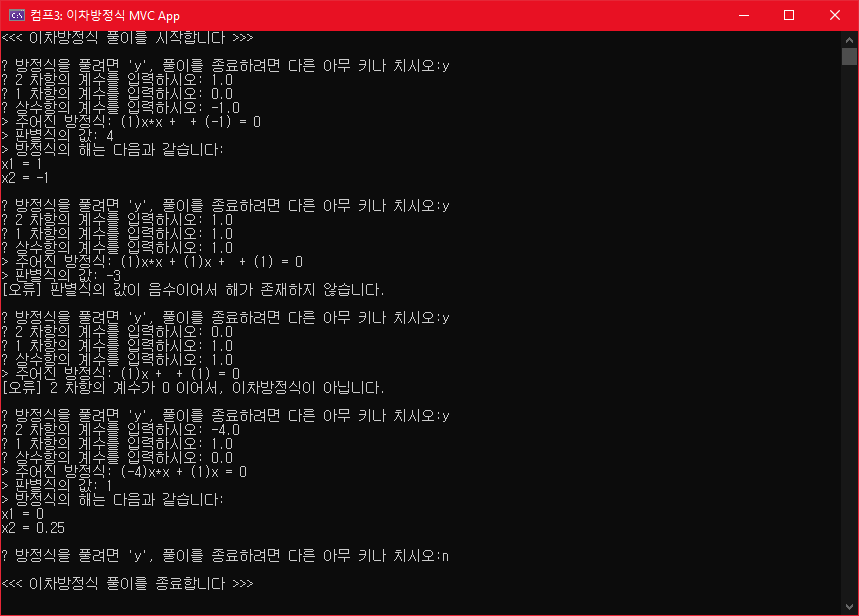
\includegraphics[width=\textwidth]{test_result.png}
        \section{입력과 출력}
            실습 자료에서 제시된 입력을 사용하였으며 모든 경우에 대해 정상적으로 처리됨을 확인하였음.
        \section{결과 분석}
            실습 자료에서 제시된 출력과 동일함을 확인하였음.

    \chapter{소스코드}
        소스코드는 제출된 압축파일에 같이 동봉되어있으며 GitHub (0x00000FF/CNUCSE-Computer-Programming-III-2020-Spring) 에서도 열람할 수 있다.
\end{document}